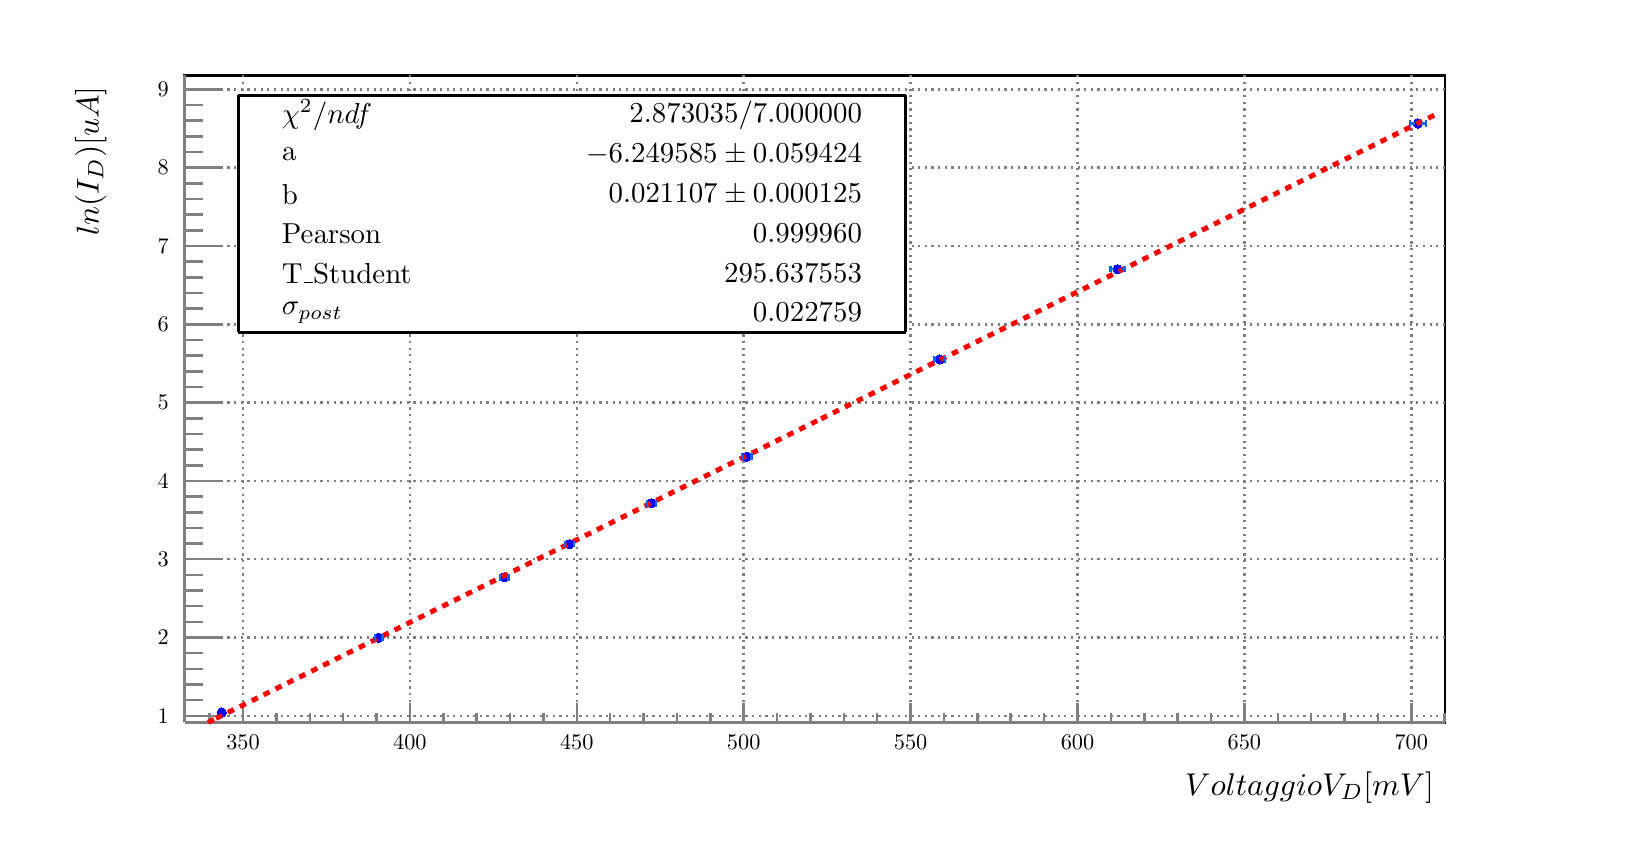
\begin{tikzpicture}
\pgfdeclareplotmark{cross} {
\pgfpathmoveto{\pgfpoint{-0.3\pgfplotmarksize}{\pgfplotmarksize}}
\pgfpathlineto{\pgfpoint{+0.3\pgfplotmarksize}{\pgfplotmarksize}}
\pgfpathlineto{\pgfpoint{+0.3\pgfplotmarksize}{0.3\pgfplotmarksize}}
\pgfpathlineto{\pgfpoint{+1\pgfplotmarksize}{0.3\pgfplotmarksize}}
\pgfpathlineto{\pgfpoint{+1\pgfplotmarksize}{-0.3\pgfplotmarksize}}
\pgfpathlineto{\pgfpoint{+0.3\pgfplotmarksize}{-0.3\pgfplotmarksize}}
\pgfpathlineto{\pgfpoint{+0.3\pgfplotmarksize}{-1.\pgfplotmarksize}}
\pgfpathlineto{\pgfpoint{-0.3\pgfplotmarksize}{-1.\pgfplotmarksize}}
\pgfpathlineto{\pgfpoint{-0.3\pgfplotmarksize}{-0.3\pgfplotmarksize}}
\pgfpathlineto{\pgfpoint{-1.\pgfplotmarksize}{-0.3\pgfplotmarksize}}
\pgfpathlineto{\pgfpoint{-1.\pgfplotmarksize}{0.3\pgfplotmarksize}}
\pgfpathlineto{\pgfpoint{-0.3\pgfplotmarksize}{0.3\pgfplotmarksize}}
\pgfpathclose
\pgfusepathqstroke
}
\pgfdeclareplotmark{cross*} {
\pgfpathmoveto{\pgfpoint{-0.3\pgfplotmarksize}{\pgfplotmarksize}}
\pgfpathlineto{\pgfpoint{+0.3\pgfplotmarksize}{\pgfplotmarksize}}
\pgfpathlineto{\pgfpoint{+0.3\pgfplotmarksize}{0.3\pgfplotmarksize}}
\pgfpathlineto{\pgfpoint{+1\pgfplotmarksize}{0.3\pgfplotmarksize}}
\pgfpathlineto{\pgfpoint{+1\pgfplotmarksize}{-0.3\pgfplotmarksize}}
\pgfpathlineto{\pgfpoint{+0.3\pgfplotmarksize}{-0.3\pgfplotmarksize}}
\pgfpathlineto{\pgfpoint{+0.3\pgfplotmarksize}{-1.\pgfplotmarksize}}
\pgfpathlineto{\pgfpoint{-0.3\pgfplotmarksize}{-1.\pgfplotmarksize}}
\pgfpathlineto{\pgfpoint{-0.3\pgfplotmarksize}{-0.3\pgfplotmarksize}}
\pgfpathlineto{\pgfpoint{-1.\pgfplotmarksize}{-0.3\pgfplotmarksize}}
\pgfpathlineto{\pgfpoint{-1.\pgfplotmarksize}{0.3\pgfplotmarksize}}
\pgfpathlineto{\pgfpoint{-0.3\pgfplotmarksize}{0.3\pgfplotmarksize}}
\pgfpathclose
\pgfusepathqfillstroke
}
\pgfdeclareplotmark{newstar} {
\pgfpathmoveto{\pgfqpoint{0pt}{\pgfplotmarksize}}
\pgfpathlineto{\pgfqpointpolar{44}{0.5\pgfplotmarksize}}
\pgfpathlineto{\pgfqpointpolar{18}{\pgfplotmarksize}}
\pgfpathlineto{\pgfqpointpolar{-20}{0.5\pgfplotmarksize}}
\pgfpathlineto{\pgfqpointpolar{-54}{\pgfplotmarksize}}
\pgfpathlineto{\pgfqpointpolar{-90}{0.5\pgfplotmarksize}}
\pgfpathlineto{\pgfqpointpolar{234}{\pgfplotmarksize}}
\pgfpathlineto{\pgfqpointpolar{198}{0.5\pgfplotmarksize}}
\pgfpathlineto{\pgfqpointpolar{162}{\pgfplotmarksize}}
\pgfpathlineto{\pgfqpointpolar{134}{0.5\pgfplotmarksize}}
\pgfpathclose
\pgfusepathqstroke
}
\pgfdeclareplotmark{newstar*} {
\pgfpathmoveto{\pgfqpoint{0pt}{\pgfplotmarksize}}
\pgfpathlineto{\pgfqpointpolar{44}{0.5\pgfplotmarksize}}
\pgfpathlineto{\pgfqpointpolar{18}{\pgfplotmarksize}}
\pgfpathlineto{\pgfqpointpolar{-20}{0.5\pgfplotmarksize}}
\pgfpathlineto{\pgfqpointpolar{-54}{\pgfplotmarksize}}
\pgfpathlineto{\pgfqpointpolar{-90}{0.5\pgfplotmarksize}}
\pgfpathlineto{\pgfqpointpolar{234}{\pgfplotmarksize}}
\pgfpathlineto{\pgfqpointpolar{198}{0.5\pgfplotmarksize}}
\pgfpathlineto{\pgfqpointpolar{162}{\pgfplotmarksize}}
\pgfpathlineto{\pgfqpointpolar{134}{0.5\pgfplotmarksize}}
\pgfpathclose
\pgfusepathqfillstroke
}
\definecolor{c}{rgb}{1,1,1};
\draw [color=c, fill=c] (0,0) rectangle (20,10.2882);
\draw [color=c, fill=c] (1.98506,1.47279) rectangle (17.9936,9.6905);
\definecolor{c}{rgb}{0,0,0};
\draw [c,line width=0.9] (1.98506,1.47279) -- (1.98506,9.6905) -- (17.9936,9.6905) -- (17.9936,1.47279) -- (1.98506,1.47279);
\definecolor{c}{rgb}{1,1,1};
\draw [color=c, fill=c] (1.98506,1.47279) rectangle (17.9936,9.6905);
\definecolor{c}{rgb}{0,0,0};
\draw [c,line width=0.9] (1.98506,1.47279) -- (1.98506,9.6905) -- (17.9936,9.6905) -- (17.9936,1.47279) -- (1.98506,1.47279);
\definecolor{c}{rgb}{0.5,0.5,0.5};
\draw [c,line width=0.9] (1.98506,1.47279) -- (17.9936,1.47279);
\draw [c,dash pattern=on 0.80pt off 1.60pt ,line width=0.9] (2.72803,9.6905) -- (2.72803,1.47279);
\draw [c,dash pattern=on 0.80pt off 1.60pt ,line width=0.9] (4.84754,9.6905) -- (4.84754,1.47279);
\draw [c,dash pattern=on 0.80pt off 1.60pt ,line width=0.9] (6.96705,9.6905) -- (6.96705,1.47279);
\draw [c,dash pattern=on 0.80pt off 1.60pt ,line width=0.9] (9.08656,9.6905) -- (9.08656,1.47279);
\draw [c,dash pattern=on 0.80pt off 1.60pt ,line width=0.9] (11.2061,9.6905) -- (11.2061,1.47279);
\draw [c,dash pattern=on 0.80pt off 1.60pt ,line width=0.9] (13.3256,9.6905) -- (13.3256,1.47279);
\draw [c,dash pattern=on 0.80pt off 1.60pt ,line width=0.9] (15.4451,9.6905) -- (15.4451,1.47279);
\draw [c,dash pattern=on 0.80pt off 1.60pt ,line width=0.9] (17.5646,9.6905) -- (17.5646,1.47279);
\draw [c,dash pattern=on 0.80pt off 1.60pt ,line width=0.9] (2.72803,9.6905) -- (2.72803,1.47279);
\draw [c,dash pattern=on 0.80pt off 1.60pt ,line width=0.9] (17.5646,9.6905) -- (17.5646,1.47279);
\draw [c,line width=0.9] (1.98506,1.47279) -- (1.98506,9.6905);
\draw [c,dash pattern=on 0.80pt off 1.60pt ,line width=0.9] (17.9936,1.55515) -- (1.98506,1.55515);
\draw [c,dash pattern=on 0.80pt off 1.60pt ,line width=0.9] (17.9936,2.54963) -- (1.98506,2.54963);
\draw [c,dash pattern=on 0.80pt off 1.60pt ,line width=0.9] (17.9936,3.54411) -- (1.98506,3.54411);
\draw [c,dash pattern=on 0.80pt off 1.60pt ,line width=0.9] (17.9936,4.53859) -- (1.98506,4.53859);
\draw [c,dash pattern=on 0.80pt off 1.60pt ,line width=0.9] (17.9936,5.53307) -- (1.98506,5.53307);
\draw [c,dash pattern=on 0.80pt off 1.60pt ,line width=0.9] (17.9936,6.52755) -- (1.98506,6.52755);
\draw [c,dash pattern=on 0.80pt off 1.60pt ,line width=0.9] (17.9936,7.52203) -- (1.98506,7.52203);
\draw [c,dash pattern=on 0.80pt off 1.60pt ,line width=0.9] (17.9936,8.51651) -- (1.98506,8.51651);
\draw [c,dash pattern=on 0.80pt off 1.60pt ,line width=0.9] (17.9936,9.51099) -- (1.98506,9.51099);
\draw [c,dash pattern=on 0.80pt off 1.60pt ,line width=0.9] (17.9936,1.55515) -- (1.98506,1.55515);
\draw [c,dash pattern=on 0.80pt off 1.60pt ,line width=0.9] (17.9936,9.51099) -- (1.98506,9.51099);
\draw [c,line width=0.9] (1.98506,1.47279) -- (17.9936,1.47279);
\draw [c,line width=0.9] (2.72803,1.71983) -- (2.72803,1.47279);
\draw [c,line width=0.9] (3.15194,1.59631) -- (3.15194,1.47279);
\draw [c,line width=0.9] (3.57584,1.59631) -- (3.57584,1.47279);
\draw [c,line width=0.9] (3.99974,1.59631) -- (3.99974,1.47279);
\draw [c,line width=0.9] (4.42364,1.59631) -- (4.42364,1.47279);
\draw [c,line width=0.9] (4.84754,1.71983) -- (4.84754,1.47279);
\draw [c,line width=0.9] (5.27145,1.59631) -- (5.27145,1.47279);
\draw [c,line width=0.9] (5.69535,1.59631) -- (5.69535,1.47279);
\draw [c,line width=0.9] (6.11925,1.59631) -- (6.11925,1.47279);
\draw [c,line width=0.9] (6.54315,1.59631) -- (6.54315,1.47279);
\draw [c,line width=0.9] (6.96705,1.71983) -- (6.96705,1.47279);
\draw [c,line width=0.9] (7.39096,1.59631) -- (7.39096,1.47279);
\draw [c,line width=0.9] (7.81486,1.59631) -- (7.81486,1.47279);
\draw [c,line width=0.9] (8.23876,1.59631) -- (8.23876,1.47279);
\draw [c,line width=0.9] (8.66266,1.59631) -- (8.66266,1.47279);
\draw [c,line width=0.9] (9.08656,1.71983) -- (9.08656,1.47279);
\draw [c,line width=0.9] (9.51047,1.59631) -- (9.51047,1.47279);
\draw [c,line width=0.9] (9.93437,1.59631) -- (9.93437,1.47279);
\draw [c,line width=0.9] (10.3583,1.59631) -- (10.3583,1.47279);
\draw [c,line width=0.9] (10.7822,1.59631) -- (10.7822,1.47279);
\draw [c,line width=0.9] (11.2061,1.71983) -- (11.2061,1.47279);
\draw [c,line width=0.9] (11.63,1.59631) -- (11.63,1.47279);
\draw [c,line width=0.9] (12.0539,1.59631) -- (12.0539,1.47279);
\draw [c,line width=0.9] (12.4778,1.59631) -- (12.4778,1.47279);
\draw [c,line width=0.9] (12.9017,1.59631) -- (12.9017,1.47279);
\draw [c,line width=0.9] (13.3256,1.71983) -- (13.3256,1.47279);
\draw [c,line width=0.9] (13.7495,1.59631) -- (13.7495,1.47279);
\draw [c,line width=0.9] (14.1734,1.59631) -- (14.1734,1.47279);
\draw [c,line width=0.9] (14.5973,1.59631) -- (14.5973,1.47279);
\draw [c,line width=0.9] (15.0212,1.59631) -- (15.0212,1.47279);
\draw [c,line width=0.9] (15.4451,1.71983) -- (15.4451,1.47279);
\draw [c,line width=0.9] (15.869,1.59631) -- (15.869,1.47279);
\draw [c,line width=0.9] (16.2929,1.59631) -- (16.2929,1.47279);
\draw [c,line width=0.9] (16.7168,1.59631) -- (16.7168,1.47279);
\draw [c,line width=0.9] (17.1407,1.59631) -- (17.1407,1.47279);
\draw [c,line width=0.9] (17.5646,1.71983) -- (17.5646,1.47279);
\draw [c,line width=0.9] (2.72803,1.71983) -- (2.72803,1.47279);
\draw [c,line width=0.9] (2.30413,1.59631) -- (2.30413,1.47279);
\draw [c,line width=0.9] (17.5646,1.71983) -- (17.5646,1.47279);
\draw [c,line width=0.9] (17.9885,1.59631) -- (17.9885,1.47279);
\definecolor{c}{rgb}{0,0,0};
\draw [anchor=base] (2.72803,1.13328) node[scale=0.805902, color=c, rotate=0]{350};
\draw [anchor=base] (4.84754,1.13328) node[scale=0.805902, color=c, rotate=0]{400};
\draw [anchor=base] (6.96705,1.13328) node[scale=0.805902, color=c, rotate=0]{450};
\draw [anchor=base] (9.08656,1.13328) node[scale=0.805902, color=c, rotate=0]{500};
\draw [anchor=base] (11.2061,1.13328) node[scale=0.805902, color=c, rotate=0]{550};
\draw [anchor=base] (13.3256,1.13328) node[scale=0.805902, color=c, rotate=0]{600};
\draw [anchor=base] (15.4451,1.13328) node[scale=0.805902, color=c, rotate=0]{650};
\draw [anchor=base] (17.5646,1.13328) node[scale=0.805902, color=c, rotate=0]{700};
\draw [anchor= east] (17.9936,0.649733) node[scale=1.13774, color=c, rotate=0]{$Voltaggio V_{D} [mV]$};
\definecolor{c}{rgb}{0.5,0.5,0.5};
\draw [c,line width=0.9] (1.98506,1.47279) -- (1.98506,9.6905);
\draw [c,line width=0.9] (2.46431,1.55515) -- (1.98506,1.55515);
\draw [c,line width=0.9] (2.22469,1.75405) -- (1.98506,1.75405);
\draw [c,line width=0.9] (2.22469,1.95295) -- (1.98506,1.95295);
\draw [c,line width=0.9] (2.22469,2.15184) -- (1.98506,2.15184);
\draw [c,line width=0.9] (2.22469,2.35074) -- (1.98506,2.35074);
\draw [c,line width=0.9] (2.46431,2.54963) -- (1.98506,2.54963);
\draw [c,line width=0.9] (2.22469,2.74853) -- (1.98506,2.74853);
\draw [c,line width=0.9] (2.22469,2.94743) -- (1.98506,2.94743);
\draw [c,line width=0.9] (2.22469,3.14632) -- (1.98506,3.14632);
\draw [c,line width=0.9] (2.22469,3.34522) -- (1.98506,3.34522);
\draw [c,line width=0.9] (2.46431,3.54411) -- (1.98506,3.54411);
\draw [c,line width=0.9] (2.22469,3.74301) -- (1.98506,3.74301);
\draw [c,line width=0.9] (2.22469,3.94191) -- (1.98506,3.94191);
\draw [c,line width=0.9] (2.22469,4.1408) -- (1.98506,4.1408);
\draw [c,line width=0.9] (2.22469,4.3397) -- (1.98506,4.3397);
\draw [c,line width=0.9] (2.46431,4.53859) -- (1.98506,4.53859);
\draw [c,line width=0.9] (2.22469,4.73749) -- (1.98506,4.73749);
\draw [c,line width=0.9] (2.22469,4.93639) -- (1.98506,4.93639);
\draw [c,line width=0.9] (2.22469,5.13528) -- (1.98506,5.13528);
\draw [c,line width=0.9] (2.22469,5.33418) -- (1.98506,5.33418);
\draw [c,line width=0.9] (2.46431,5.53307) -- (1.98506,5.53307);
\draw [c,line width=0.9] (2.22469,5.73197) -- (1.98506,5.73197);
\draw [c,line width=0.9] (2.22469,5.93087) -- (1.98506,5.93087);
\draw [c,line width=0.9] (2.22469,6.12976) -- (1.98506,6.12976);
\draw [c,line width=0.9] (2.22469,6.32866) -- (1.98506,6.32866);
\draw [c,line width=0.9] (2.46431,6.52755) -- (1.98506,6.52755);
\draw [c,line width=0.9] (2.22469,6.72645) -- (1.98506,6.72645);
\draw [c,line width=0.9] (2.22469,6.92534) -- (1.98506,6.92534);
\draw [c,line width=0.9] (2.22469,7.12424) -- (1.98506,7.12424);
\draw [c,line width=0.9] (2.22469,7.32314) -- (1.98506,7.32314);
\draw [c,line width=0.9] (2.46431,7.52203) -- (1.98506,7.52203);
\draw [c,line width=0.9] (2.22469,7.72093) -- (1.98506,7.72093);
\draw [c,line width=0.9] (2.22469,7.91982) -- (1.98506,7.91982);
\draw [c,line width=0.9] (2.22469,8.11872) -- (1.98506,8.11872);
\draw [c,line width=0.9] (2.22469,8.31762) -- (1.98506,8.31762);
\draw [c,line width=0.9] (2.46431,8.51651) -- (1.98506,8.51651);
\draw [c,line width=0.9] (2.22469,8.71541) -- (1.98506,8.71541);
\draw [c,line width=0.9] (2.22469,8.9143) -- (1.98506,8.9143);
\draw [c,line width=0.9] (2.22469,9.1132) -- (1.98506,9.1132);
\draw [c,line width=0.9] (2.22469,9.3121) -- (1.98506,9.3121);
\draw [c,line width=0.9] (2.46431,9.51099) -- (1.98506,9.51099);
\draw [c,line width=0.9] (2.46431,1.55515) -- (1.98506,1.55515);
\draw [c,line width=0.9] (2.46431,9.51099) -- (1.98506,9.51099);
\definecolor{c}{rgb}{0,0,0};
\draw [anchor= east] (1.88506,1.55515) node[scale=0.805902, color=c, rotate=0]{1};
\draw [anchor= east] (1.88506,2.54963) node[scale=0.805902, color=c, rotate=0]{2};
\draw [anchor= east] (1.88506,3.54411) node[scale=0.805902, color=c, rotate=0]{3};
\draw [anchor= east] (1.88506,4.53859) node[scale=0.805902, color=c, rotate=0]{4};
\draw [anchor= east] (1.88506,5.53307) node[scale=0.805902, color=c, rotate=0]{5};
\draw [anchor= east] (1.88506,6.52755) node[scale=0.805902, color=c, rotate=0]{6};
\draw [anchor= east] (1.88506,7.52203) node[scale=0.805902, color=c, rotate=0]{7};
\draw [anchor= east] (1.88506,8.51651) node[scale=0.805902, color=c, rotate=0]{8};
\draw [anchor= east] (1.88506,9.51099) node[scale=0.805902, color=c, rotate=0]{9};
\draw [anchor= east] (0.792956,9.6905) node[scale=1.13774, color=c, rotate=90]{$ln(I_{D}) [uA]$};
\definecolor{c}{rgb}{0,0,1};
\foreach \P in {(2.45674,1.59872), (4.44908,2.54841), (6.04719,3.31609), (6.8738,3.73681), (7.91659,4.25569), (9.12471,4.84674), (11.5749,6.08194), (13.8343,7.22866), (17.6494,9.07937)}{\draw[mark options={color=c,fill=c},mark size=1.681682pt, line
 width=0.000000pt, mark=*] plot coordinates {\P};}
\definecolor{c}{rgb}{1,0,0};
\draw [c,dash pattern=on 2.40pt off 2.40pt ,line width=1.8] (2.28453,1.47279) -- (2.38527,1.52267);
\draw [c,dash pattern=on 2.40pt off 2.40pt ,line width=1.8] (2.38527,1.52267) -- (2.54536,1.60194) -- (2.70544,1.68122) -- (2.86553,1.76049) -- (3.02561,1.83976) -- (3.1857,1.91903) -- (3.34578,1.9983) -- (3.50587,2.07757) -- (3.66596,2.15685) --
 (3.82604,2.23612) -- (3.98613,2.31539) -- (4.14621,2.39466) -- (4.3063,2.47393) -- (4.46638,2.5532) -- (4.62647,2.63247) -- (4.78655,2.71175) -- (4.94664,2.79102) -- (5.10672,2.87029) -- (5.26681,2.94956) -- (5.42689,3.02883) -- (5.58698,3.1081) --
 (5.74707,3.18738) -- (5.90715,3.26665) -- (6.06724,3.34592) -- (6.22732,3.42519) -- (6.38741,3.50446) -- (6.54749,3.58373) -- (6.70758,3.663) -- (6.86766,3.74228) -- (7.02775,3.82155) -- (7.18783,3.90082) -- (7.34792,3.98009) -- (7.508,4.05936) --
 (7.66809,4.13863) -- (7.82818,4.21791) -- (7.98826,4.29718) -- (8.14835,4.37645) -- (8.30843,4.45572) -- (8.46852,4.53499) -- (8.6286,4.61426) -- (8.78869,4.69353) -- (8.94877,4.77281) -- (9.10886,4.85208) -- (9.26894,4.93135) -- (9.42903,5.01062)
 -- (9.58911,5.08989) -- (9.7492,5.16916) -- (9.90928,5.24843) -- (10.0694,5.32771);
\draw [c,dash pattern=on 2.40pt off 2.40pt ,line width=1.8] (10.0694,5.32771) -- (10.2295,5.40698) -- (10.3895,5.48625) -- (10.5496,5.56552) -- (10.7097,5.64479) -- (10.8698,5.72406) -- (11.0299,5.80334) -- (11.19,5.88261) -- (11.3501,5.96188) --
 (11.5101,6.04115) -- (11.6702,6.12042) -- (11.8303,6.19969) -- (11.9904,6.27896) -- (12.1505,6.35824) -- (12.3106,6.43751) -- (12.4707,6.51678) -- (12.6307,6.59605) -- (12.7908,6.67532) -- (12.9509,6.75459) -- (13.111,6.83387) -- (13.2711,6.91314)
 -- (13.4312,6.99241) -- (13.5912,7.07168) -- (13.7513,7.15095) -- (13.9114,7.23022) -- (14.0715,7.30949) -- (14.2316,7.38877) -- (14.3917,7.46804) -- (14.5518,7.54731) -- (14.7118,7.62658) -- (14.8719,7.70585) -- (15.032,7.78512) --
 (15.1921,7.86439) -- (15.3522,7.94367) -- (15.5123,8.02294) -- (15.6724,8.10221) -- (15.8324,8.18148) -- (15.9925,8.26075) -- (16.1526,8.34002) -- (16.3127,8.4193) -- (16.4728,8.49857) -- (16.6329,8.57784) -- (16.793,8.65711) -- (16.953,8.73638) --
 (17.1131,8.81565) -- (17.2732,8.89492) -- (17.4333,8.9742) -- (17.5934,9.05347) -- (17.7535,9.13274) -- (17.9136,9.21201);
\definecolor{c}{rgb}{0,0.4,1};
\draw [c,line width=0.9] (4.40639,2.54841) -- (4.40103,2.54841);
\draw [c,line width=0.9] (4.40103,2.50573) -- (4.40103,2.5911);
\draw [c,line width=0.9] (4.49177,2.54841) -- (4.49712,2.54841);
\draw [c,line width=0.9] (4.49712,2.50573) -- (4.49712,2.5911);
\draw [c,line width=0.9] (6.0045,3.31609) -- (5.99455,3.31609);
\draw [c,line width=0.9] (5.99455,3.2734) -- (5.99455,3.35878);
\draw [c,line width=0.9] (6.08988,3.31609) -- (6.09983,3.31609);
\draw [c,line width=0.9] (6.09983,3.2734) -- (6.09983,3.35878);
\draw [c,line width=0.9] (6.83111,3.73681) -- (6.81878,3.73681);
\draw [c,line width=0.9] (6.81878,3.69412) -- (6.81878,3.7795);
\draw [c,line width=0.9] (6.91648,3.73681) -- (6.92881,3.73681);
\draw [c,line width=0.9] (6.92881,3.69412) -- (6.92881,3.7795);
\draw [c,line width=0.9] (7.87391,4.25569) -- (7.85858,4.25569);
\draw [c,line width=0.9] (7.85858,4.213) -- (7.85858,4.29838);
\draw [c,line width=0.9] (7.95928,4.25569) -- (7.97461,4.25569);
\draw [c,line width=0.9] (7.97461,4.213) -- (7.97461,4.29838);
\draw [c,line width=0.9] (9.08203,4.84674) -- (9.06322,4.84674);
\draw [c,line width=0.9] (9.06322,4.80405) -- (9.06322,4.88943);
\draw [c,line width=0.9] (9.16741,4.84674) -- (9.18621,4.84674);
\draw [c,line width=0.9] (9.18621,4.80405) -- (9.18621,4.88943);
\draw [c,line width=0.9] (11.5322,6.08194) -- (11.5063,6.08194);
\draw [c,line width=0.9] (11.5063,6.03925) -- (11.5063,6.12463);
\draw [c,line width=0.9] (11.6176,6.08194) -- (11.6434,6.08194);
\draw [c,line width=0.9] (11.6434,6.03925) -- (11.6434,6.12463);
\draw [c,line width=0.9] (13.7916,7.22866) -- (13.7448,7.22866);
\draw [c,line width=0.9] (13.7448,7.18597) -- (13.7448,7.27135);
\draw [c,line width=0.9] (13.877,7.22866) -- (13.9237,7.22866);
\draw [c,line width=0.9] (13.9237,7.18597) -- (13.9237,7.27135);
\draw [c,line width=0.9] (17.6067,9.07937) -- (17.5505,9.07937);
\draw [c,line width=0.9] (17.5505,9.03668) -- (17.5505,9.12206);
\draw [c,line width=0.9] (17.6921,9.07937) -- (17.7483,9.07937);
\draw [c,line width=0.9] (17.7483,9.03668) -- (17.7483,9.12206);
\definecolor{c}{rgb}{1,1,1};
\draw [color=c, fill=c] (2.66809,6.42476) rectangle (11.1419,9.43437);
\definecolor{c}{rgb}{0,0,0};
\draw [c,line width=0.9] (2.66809,6.42476) -- (11.1419,6.42476);
\draw [c,line width=0.9] (11.1419,6.42476) -- (11.1419,9.43437);
\draw [c,line width=0.9] (11.1419,9.43437) -- (2.66809,9.43437);
\draw [c,line width=0.9] (2.66809,9.43437) -- (2.66809,6.42476);
\draw [anchor= west] (3.09178,9.18356) node[scale=1.04293, color=c, rotate=0]{$\chi^{2} / ndf $};
\draw [anchor= east] (10.7182,9.18356) node[scale=1.04293, color=c, rotate=0]{2.873035/7.000000};
\draw [anchor= west] (3.09178,8.68196) node[scale=1.04293, color=c, rotate=0]{a        };
\draw [anchor= east] (10.7182,8.68196) node[scale=1.04293, color=c, rotate=0]{$ -6.249585\pm0.059424$};
\draw [anchor= west] (3.09178,8.18036) node[scale=1.04293, color=c, rotate=0]{b        };
\draw [anchor= east] (10.7182,8.18036) node[scale=1.04293, color=c, rotate=0]{$ 0.021107\pm0.000125$};
\draw [anchor= west] (3.09178,7.67876) node[scale=1.04293, color=c, rotate=0]{Pearson        };
\draw [anchor= east] (10.7182,7.67876) node[scale=1.04293, color=c, rotate=0]{ 0.999960};
\draw [anchor= west] (3.09178,7.17716) node[scale=1.04293, color=c, rotate=0]{T\_Student        };
\draw [anchor= east] (10.7182,7.17716) node[scale=1.04293, color=c, rotate=0]{ 295.637553};
\draw [anchor= west] (3.09178,6.67556) node[scale=1.04293, color=c, rotate=0]{$\sigma_{post}        $};
\draw [anchor= east] (10.7182,6.67556) node[scale=1.04293, color=c, rotate=0]{ 0.022759};
\end{tikzpicture}
